\chapter{Dynamism in compiler frameworks}
\label{chap:dynamism-pattern-rewriting}

%% Introduction
% Hook
A key difference between the Python and C++ runtimes is their degree of dynamism.
% Argument
\ac{mlir}'s C++ runtime incurs overhead when dynamically dispatching functions (\autoref{fig:narrative}, \circledbase{pairedThreeLightGreen}{3}), which is worsened by prohibiting ahead-of-time performance optimisations.
In contrast, Python dynamically evaluates each bytecode operation individually in its interpreter loop, incurring an overhead each time. % OLD: In contrast, almost every bytecode operation evaluated by the Python interpreter is dynamic, each incurring an overhead.
As such, we expect the difference in performance between language runtimes (\autoref{fig:narrative}, \circledbase{pairedFourDarkGreen}{4}) to be smaller for more dynamic workloads.
% Link
In this chapter, we quantify this difference by examining synthetic examples within static and dynamic language runtimes. We then apply this information to understand the difference in performance between pattern rewriting workloads using xDSL and \ac{mlir} through the lens of overhead incurred by dynamism.


\section{Cost of dynamic dispatch}
\label{sec:dynamism-pattern-rewriting-dispatch}

%% Introduce the issue, and where it is in the micro-benchmark
% Hook
In static languages such as C++, the exact address function calls can often be resolved at compile time. In contrast, dynamic languages such as Python must resolve the address of each function call at runtime, incurring an overhead.
% Also optimisation boundary and stuff
% Argument
However, the address of some function calls can only be known at runtime, for example as a result of object polymorphism. This address then must be resolved during execution by the language runtime in both static and dynamic languages. Furthermore, this information being known only at runtime presents an optimisation boundary, precluding common rewrites such as function inlining which contribute to the performance of ahead-of-time compiled languages.
Driesen and H\"olzle quantify the former and acknowledge the latter cost in their work ``The Direct Cost of Virtual Function Calls in C++'' \cite{driesenDirectCostVirtual1996}, which found that C++ programs spent a median of $5.2\%$ of their time in dispatch code. % TODO: Possibly pick a different metric from the paper, and lift to related work!
We argue further that the difference between static and dynamic languages is reduced for highly dynamic workloads with insufficient information to resolve function addresses ahead of time.
% Link
We justify this by examining the mechanisms of dynamic dispatch in Python and C++, and contrasting them through both synthetic examples and our micro-benchmark suite.

% Hook
% Argument
C++ uses a \ac{vtable} mechanism for method polymorphism, a lookup table which is accessed at runtime through pointer indirection to retrieve the address for the virtual function implementation. In contrast, Python stores methods and attributes in the \mintinline{text}{__dict__} object attribute which is searched at runtime, checking parent classes if needed. While both use indirection for dynamic dispatch, Python's approach enables more dynamic behaviour like runtime meta-programming but comes with higher performance costs compared to C++'s more efficient \ac{vtable} system.
% Link
We can quantify the performance overhead of this \ac{vtable} mechanism through a synthetic example (Listing \ref{listing:impact-dispatch}).


\begin{figure}[H]
    \centering
    \begin{subfigure}[b]{0.45\textwidth}
       \centering
        \begin{minted}[fontsize=\scriptsize,escapeinside=££]{text}
class Base {
public:
    int func(int a, int b) { £\circledbase{pairedTwoDarkBlue}{\scriptsize{b}}£
        return a - b;
    }
    __attribute__((noinline))
    int uninlinedFunc(int a, int b) { £\circledbase{pairedThreeLightGreen}{\scriptsize{e}}£
        return a - b;
    }
    virtual int virtualFunc(int a, int b) { £\circledbase{pairedFourDarkGreen}{\scriptsize{a}}£
        return a - b;
    }
};

class Derived : public Base {
public:
    int virtualFunc(int a, int b) override {
        return b - a;
    }
};
        \end{minted}
        \scriptsize{\vspace{1em}}
        \captionsetup{name=Listing}
        \caption{Method definitions.}
        \label{listing:impact-dispatch-definition}
    \end{subfigure}
    \hfill
    \begin{subfigure}[b]{0.45\textwidth}
        \centering
        \begin{minted}[breakanywhere,fontsize=\scriptsize,escapeinside=££]{text}
#include <stdlib.h>

int main(int argc, char *argv[]) {
    // Values known only at runtime £\circledbase{pairedNegOneLightGray}{\scriptsize{c}}£
    int a = atoi(argv[1]), b = atoi(argv[2]), c = atoi(argv[3]);

    // Setup
    int result = 0;
    Base baseObj;
    Derived derivedObj;
    Base* polyObj = c > 0 ? &baseObj : &derivedObj; £\circledbase{pairedNegTwoDarkGray}{\scriptsize{d}}£

    // Function invocations
    result += baseObj.func(a, b);
    result += baseObj.uninlinedFunc(a, b);
    result += polyObj->virtualFunc(a, b);

    return result;
}
        \end{minted}
        \captionsetup{name=Listing}
        \caption{Method invocations.}
        \label{listing:impact-dispatch-invocation}
    \end{subfigure}
    \vspace{1em}
    \captionsetup{name=Listing}
    \caption{Synthetic example of direct and dynamic method dispatch in C++.}
    \label{listing:impact-dispatch}
\end{figure}

% Hook
This synthetic example exercises polymorphic methods which must be resolved dynamically using a \ac{vtable} at runtime \circledbase{pairedFourDarkGreen}{\scriptsize{a}}, along with methods which can be statically resolved ahead of time during compilation \circledbase{pairedTwoDarkBlue}{\scriptsize{b}}.
% Argument
A challenge when constructing this workload is providing data whose value is known only at runtime. We implement this by taking arguments from the command line \circledbase{pairedNegOneLightGray}{\scriptsize{c}}, as opposed to defining static variables which the compiler could reason about to inform ahead of time optimisations. This is necessary to exercise dynamic dispatch of functions, which requires a polymorphic object whose type is only known at runtime \circledbase{pairedNegTwoDarkGray}{\scriptsize{d}}. Since this simple synthetic example is amenable to compiler optimisations such as function inlining, we use variable attributes to hint to the compiler that certain methods should not be inlined \circledbase{pairedThreeLightGreen}{\scriptsize{e}}.
% Link

\begin{figure}[H]
    \centering
    \begin{tikzpicture}
        \node[anchor=south west,inner sep=0] (image) at (0,0) {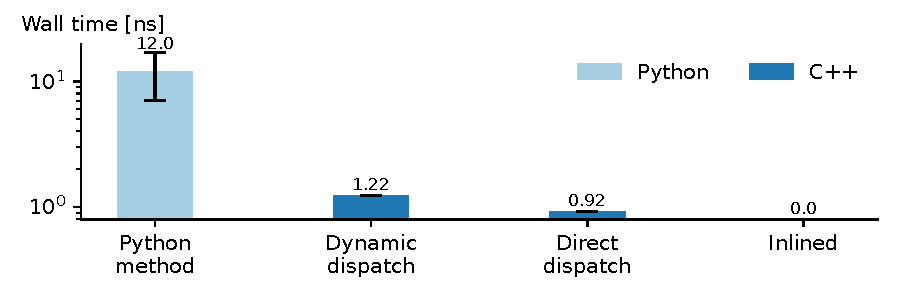
\includegraphics[width=0.75\textwidth]{images/impact_dynamism/dispatch.pdf}};
        \node[circledstyle, fill=pairedFourDarkGreen] at (4,0.625) {a};
        \node[circledstyle, fill=pairedThreeLightGreen] at (6.95,0.625) {e};
        \node[circledstyle, fill=pairedTwoDarkBlue] at (9.9,0.75) {b};
    \end{tikzpicture}
    % 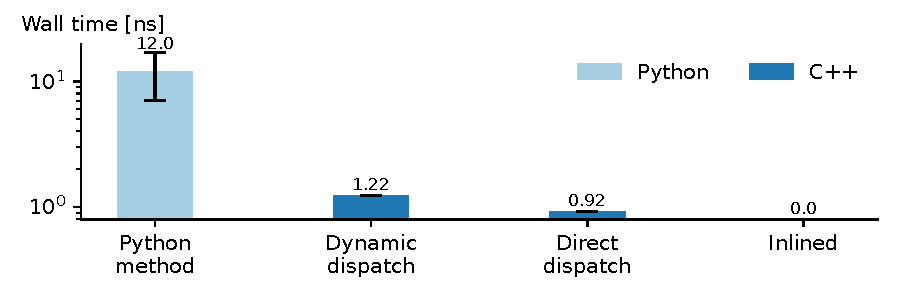
\includegraphics[width=0.75\textwidth]{images/impact_dynamism/dispatch.pdf}
    \caption{Dynamic dispatch generated by \texttt{clang -O3} incurs a $30\%$ overhead in comparison with direct dispatch, but remains an order of magnitude more performant than CPython 3.10 method invocation.}
    \label{figure:impact-dispatch}
\end{figure}


% % Hook
Having constructed this synthetic example, we calculate the cost of each method invocation by measuring the runtime of each function and subtracting the runtime of its inlined implementation (\autoref{figure:impact-dispatch}).
% % Argument
Dynamic dispatch is $30\%$ slower than direct dispatch, as a result of the overhead constructing and dereferencing through the \ac{vtable}. Examining the disassembly (\autoref{chap:impact-disassembly}), this overhead increases the instruction count from $4$ to $14$, for a total of $10$ extra cycles on ARM \ac{risc} machines. This observation matches the work of Driesen and H\"olzle, who assert the ``direct cost'' of virtual function calls is up to $10.2$ cycles for highly dynamic workloads \cite[Figure 18.]{driesenDirectCostVirtual1996}.
In addition to this Driesen and H\"olzle acknowledge there is a further ``indirect cost'' associated with hidden optimisations, but do not characterise it.
An example of such an optimisation hidden by runtime information is the inlining of the function implementation. This code motion represents the remaining $70\%$ of the overhead of dynamic dispatch -- significantly greater than the polymorphism machinery. Furthermore, this is a lower bound of this impact, as further optimisations such as vectorisation or dead code elimination could be revealed.
% Link
Despite both these direct and indirect costs, Python function invocation remains an order of magnitude slower.

%% Why is python slower?
% Hook
% Python's poor performance comes as a result of...
% Argument
% Link

% %% Where does this occur?
% Hook
Functions which can only be dispatched at runtime are one way a workload can be dynamic.
% Argument
Having a high proportion of such functions is one way in which user-extensible compiler frameworks are highly dynamic. For example, since the Operation objects composing the \ac{ir} being processed are necessarily only known at runtime, their methods such as verification and printing must be dispatched dynamically.
In other cases, \ac{mlir} is optimised to avoid this cost. For example, the \mintinline{text}{TypeID::get<Traits>} function uses template meta-programming to monomorphise the generic function calls. However, this approach is only applicable when there is sufficient information at runtime.
% Link




\section{Run-time type information}
\label{sec:dynamism-pattern-rewriting-rtti}

%% Introduce the issue
% Hook
In a ``A history of C++: 1979--1991'', Stroustop states that the original C++ design ``deliberately didn't include [mechanisms] for run-time type identification [as] they were almost always misused.'' \cite{stroustrupHistory197919911996}.
% Argument
Support for this functionality was later added in C++98 \cite{internationalorganizationforstandardizationISOIEC148821998}, including support for \texttt{dynamic\_cast}s checked a runtime, and getting the \texttt{typeid} of a polymorphic object. However, this incurs a runtime cost \cite{goldthwaite2006technical}, and is brittle in the objects to which it can be applied. A such, LLVM reimplements a subset of this functionality, providing the \texttt{dyn\_cast} method and \texttt{TypeID} data structure, aiming to ``strike a balance between performance and the setup required to enable its use'' \cite{mlirteamMLIRCodeDocumentation}.
This is another example of dynamic behaviour, which we again argue incurs additional runtime overhead and precludes optimisations in static languages, closing the gap with dynamic ones.
% Link
As before, we justify this be examining the details of this mechanism, using our micro-benchmark suite.

%% Graph
\begin{figure}[H]
    \centering
    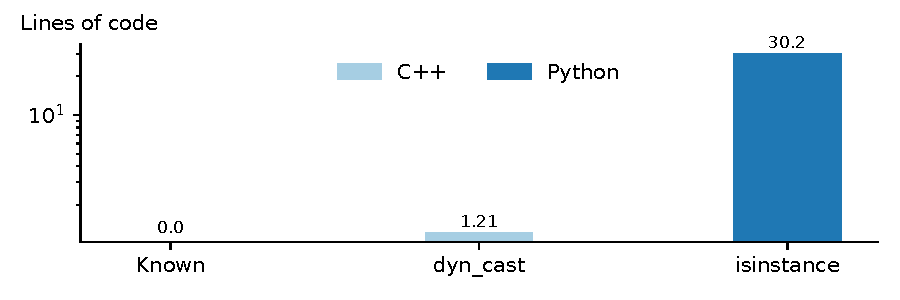
\includegraphics[width=0.75\textwidth]{images/impact_dynamism/dynamic_cast.pdf}
    \caption{Both checking and casting LLVM \ac{rtti} have a similar runtime cost, constrasting Python, which is $10\times$ slower for checking and $25\times$ slower for casting.}
    \label{figure:impact-rtti}
\end{figure}

%% Experimental results
% Hook
We measure the duration of micro-benchmarks exercising xDSL and \ac{mlir}'s \ac{rtti} operations (\autoref{figure:impact-rtti}). LLVM's \ac{rtti} implementation is much more performant than Python, leveraging C++ templates to defer as much computation as possible to compile time. In addition to this, type checking and casting have approximately the same performance cost, as they leverage similar mechanisms.
% Argument
In contrast, Python's \texttt{isinstance} function is faster than \texttt{cast}, as the former is implemented in C as a builtin function, whereas the latter is in Python in the standard library, hence relying on the dynamic dispatch machinery discussed above.
However, the implementation of the \texttt{cast} function is the identity, doing nothing unless explicitly overridden. Python's dynamic duck typing \cite{milojkovicItsDuckTyping2017} does not require restructuring data when casting, allowing casting operations and some type checks to be elided. Despite this, the \texttt{cast} function incurs a high overhead, as a result of the cost of function invocation in Python.
% Link





% % TODO: Does this want to be lifted into the dynamism section -- this might make it easier to link to more substantial data rather than just explaining interpreter/compiler again in gratuitous detail
% % Hook
% Empowered by the similarity of their implementations, we can further apply profiling tools to contrast the emitted instructions by each language runtime.
% % Argument
% For xDSL's Python, we use our novel bytecode profiling tool ByteSight, and for \ac{mlir}'s C++, we use \texttt{valgrind}'s \texttt{callgrind} tool \cite{valgrindtmdevelopersCallgrindCallgraphGenerating}.
% For the same algorithm, Python dispatches only $35$ bytecode instructions in comparison with AArch64 assembly taking $708$ (\autoref{fig:ubenchmark-original-trait-performance}).
% This demonstrates the significant abstraction gap between high-level Python bytecode and the low-level assembly instructions compiled from C++. While Python requires fewer explicit instructions due to its dynamic dispatch and built-in operations handling complex tasks internally, the underlying C++ implementation must execute many more granular assembly instructions to achieve the same computational result.
% % Link
% Despite this, the C++ implementation outperforms the Python implementation, due to these assembly instructions more closely matching the execution model of the target machine.


% \section{Object data access}
% \label{sec:dynamism-pattern-rewriting-access}

%% TODO: Depending on how re-worked the specialising chapter gets, I could add another section discussing using runtime invariants to make Python less dynamic, which would quantify __slots__


%% Contrasting with Python
% Hook
% Argument
% Link


% \section{Motivating dynamic languages for user-extensible compiler infrastructures}
\section{Dynamic languages for user-extensible compilers}
\label{chap:dynamism-pattern-rewriting-motivating}

%% Summary
% Hook
From the previous section we can see that dynamism incurs overhead and precludes ahead of time optimisations.
% Argument
This narrows the performance gap between dynamic and static languages for the implementation of this infrastructure, because the cost traditionally associated with Python's dynamic interpreted runtime is lessened by the commensurate dynamism of the user-extensible compiler framework workload. Contrasting the $60,000\times$ slowdown from C++ implementations of structured workloads such as \ac{gemm} \cite{emerybergerPythonPerformanceMatters2022}, specialised implementations of real-world xDSL workloads demonstrate Python can close this gap to only $10\times$.
In combination with developer productivity being critical for modern compiler engineers to achieve their performance goals (\autoref{chap:background}), this narrowed gap challenges the status quo of \ac{mlir} being implemented static, ahead-of-time compiled C++.
Instead, xDSL's approach of using Python improves developer productivity with its expressive syntax and fast build times, empowering fast prototypes during development.
% Link
We believe that this motivates the use of dynamic languages for the implementation of user-extensible compiler infrastructures.
